Alan Turing published his discovery of the first UTM in his original work on TM's. \cite{turing} In 1956 Claude Shannon proved that it was possible to have a UTM with only two-symbols and that it was possible to exchange the number of states with the number of symbols. \cite{two_states} His research sparked the search for the smallest possible UTM, in terms of the number of states and symbols needed to describe it. 

In 1967 Marvin Minsky found a very small UTM that needed only four symbols and seven states. \cite{minsky} in 1985 Stephen Wolfram found a smaller UTM with two states and 5 symbols. \cite{wolfram} His work, supported by Mathew Cook found a series of small UTMs, culminating in the discovery of what is currently believed to be the smallest possile UTM. Wolfram discovered a two state, three symbol TM which he believed to be a UTM. He could not, however, prove its universality. An undergraduate student, Alex Smith did prove its universality in 2007. Figure \ref{fig:23turing} shows the graphical representation that Wolfram uses to describe a TM. \cite{23turing}

\begin{figure}[!htp]
  \centering
  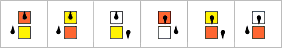
\includegraphics[width=.85\textwidth]{images/23_machine}
  \caption{The wolfram representation of the 2,3 UTM. It is the smallest possible UTM. The arrows indicate state and the colors indicate the tape symbol. Tape movement direction is shown by the left/right location of the "to state" \label{fig:23turing} }
\end{figure}

Though the majority of past research has focused on the discovery of ever smaller UTMs, this work trends in the oposite direction. Organic creatues use dna to encode their description. Feverati and Musso, in 2008, performed research using a GA to find complex TMs. Their goal was to use their model to investigate the usefullness of non-coding regions in dna encodings with regard to the creation of complex organisms. Their conclusion was that large non-coding regions, in this case represented by inaccessible states in the state-transition table, provided an evolutionary benifit.\cite{feverati-2007} This research implies that using encodings that provide a large number of possible states 